\section{Primzahlen}

\hfill \break
$P \subseteq \mathbb{N}$\\
$P = \{2,3,5,7,11,13,17,19,23,...\}$\\


Eigenschaften:
\begin{itemize}
    \item Primzahlen sind Zahlen, die nur durch Eins und durch sich selber teilbar sind.
    \item Die kleinste Primzahl ist Zwei.
\end{itemize}

\subsection{Primfaktorzerlegung}

\hfill \break
Es wird immer mit der kleisten Primzahl zerlegt.

\hfill \break
$12 = 4*3$\\
$12 = 2*2*3 = 2^2*3$\\

\hfill \break
\fboxrule=0.8pt \fcolorbox{lightgray}{lightgray}{%
    \begin{tabular}{ c|c}
        12 & 2 \\
        6  & 2 \\
        3  & 3 \\
        1  &   \\
    \end{tabular}}\\

\hfill \break
$180 = 4*9*5$\\
$180 = 2*2*3*3 = 2^2*3^2*5$\\

\hfill \break
\fboxrule=0.8pt \fcolorbox{lightgray}{lightgray}{%
    \begin{tabular}{ c|c }
        180 & 2 \\
        90  & 2 \\
        45  & 3 \\
        15  & 3 \\
        5   & 5 \\
        1   &   \\
    \end{tabular}}\\
\break
\newpage
\subsection{Größter gemeinsamer Teiler (ggt)}

Das GGT wird mittles Primfaktorzerlegung ermittelt.\\
Die Zahlen die in beiden Zerlegungen vorhanden sind werden Zusammen-multipliziert.\\

\hfill \break
Example: Ermittling des ggt von 36 und 60\\
\fboxrule=0.8pt \fcolorbox{lightgray}{lightgray}{%
    \begin{tabular}{ c|c||c|c}
        36 & \textcolor{red}{2}   & 60 & \textcolor{red}{2}   \\
        18 & \textcolor{green}{2} & 30 & \textcolor{green}{2} \\
        9  & \textcolor{blue}{3}  & 15 & \textcolor{blue}{3}  \\
        3  & 3                    & 5  & 5                    \\
        1  &                      & 1  &                      \\
    \end{tabular}}
$ggt(36,60) = \textcolor{red}{2}*\textcolor{green}{2}*\textcolor{blue}{3} = 12$
\break
\subsection{Kleinste gemeinsame Vielfache (kgv)}

\hfill \break
Das kgv wird errechnet in dem man jeden Faktor in der jeweils höchst vorkommenden Potenz miteinenader multipliziert.\\

\hfill \break
Das kgv wird wie folged berechnet:\\
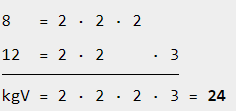
\includegraphics[scale=0.8]{KGV}

\hfill \break
Example: Ermittling des kgv von 24 und 30\\
\fboxrule=0.8pt \fcolorbox{lightgray}{lightgray}{%
    \begin{tabular}{c|c||c|c}
        24 & 2 & 30 & 2 \\
        12 & 2 & 15 & 2 \\
        6  & 2 & 5  & 5 \\
        3  & 3 & 4  &   \\
        1  &   &    &   \\
    \end{tabular}}
$kgv(24,30) = 2^3*3^1*5^1 =120$


